\subsection{Upload Album Page (Interface Mockup)}

\begin{figure}[h!]
\centering
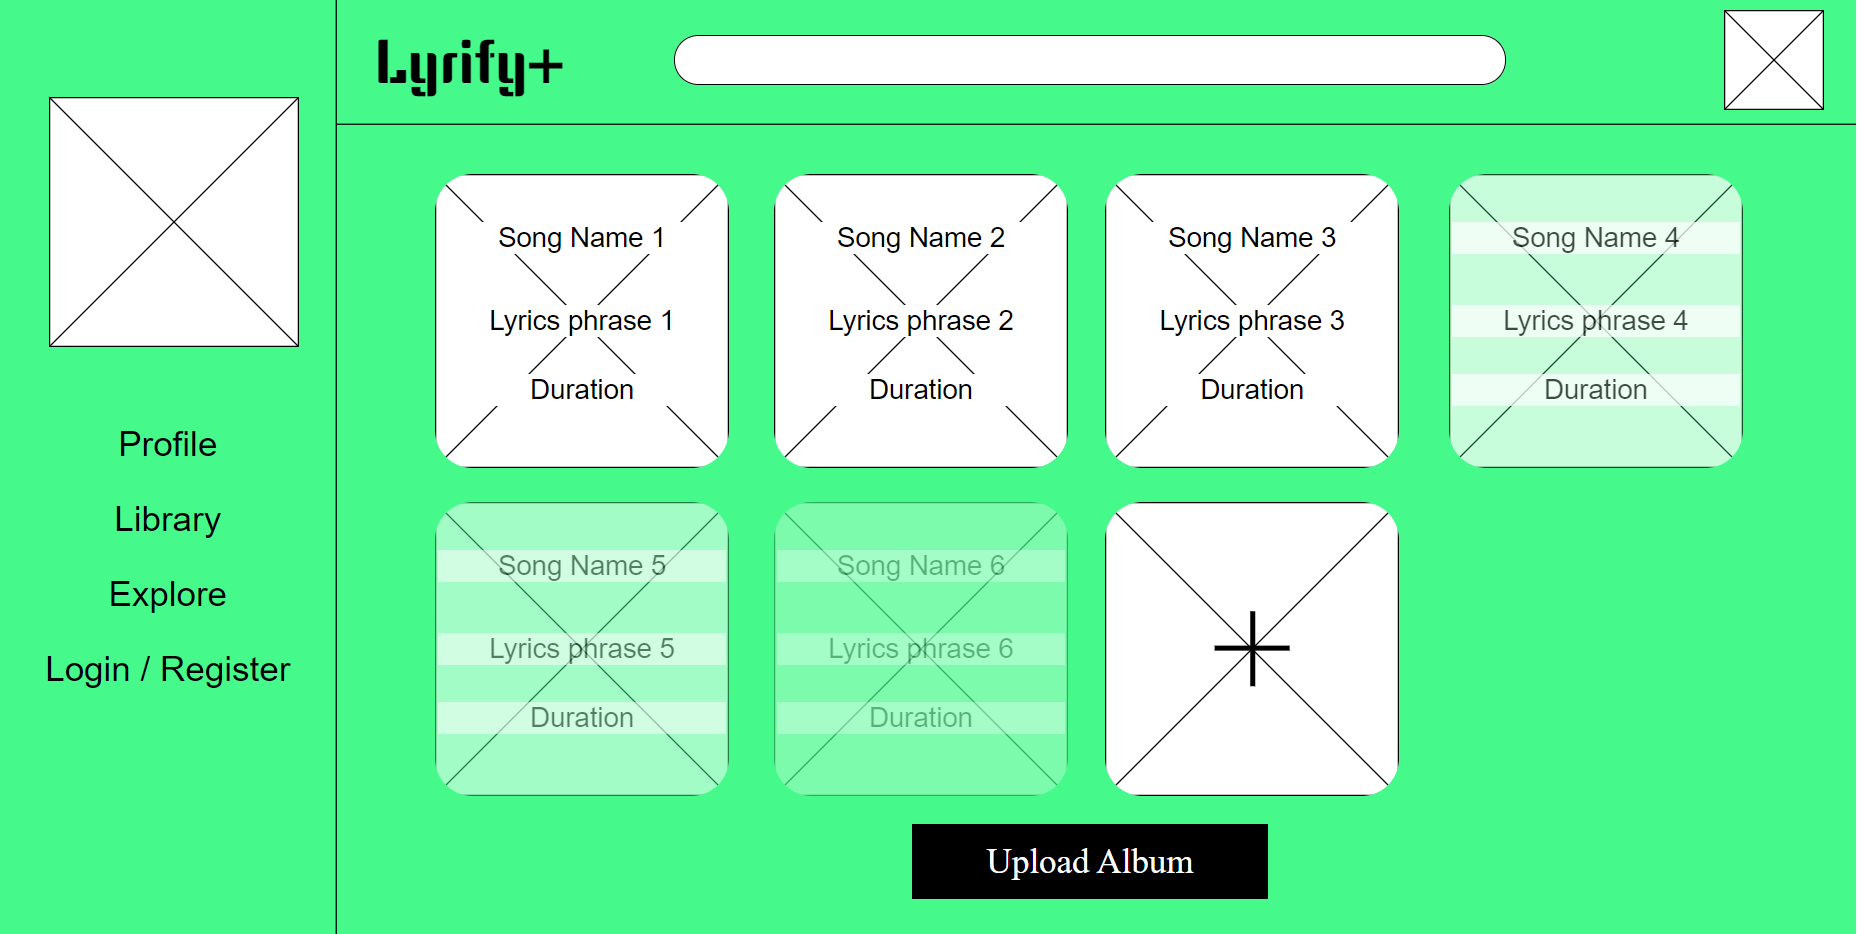
\includegraphics[width=0.9\textwidth]{sections/PLL/UploadAlbumMockUp.png}
\caption{Upload album page}
\end{figure}

This page is simpler too as it has the typical design of the others for the side and the top row. In the center of the page, we can find some squares that represents the songs added to the album. The page will begin only with the square that has a plus in the center. By clicking on it, the page will redirect you to the upload songs page in order to enter the rest of the song’s information. When done, the page will redirect you back to the album, and one square with the basic info of the song the artist just entered will be displayed, and next to it the add song square. This way the page will be filling up with the songs the artist enters. Once the album is completed, the artist will need to click on the ‘Upload album’ button to save it in our database and will be redirected to the artist’s profile page.